%!TEX root = ../DSPP.tex
\section{Hintergrund}
Motivation dieser Arbeit ist der Kurs \glqq{}M31.2 Distributed Systems and Parallel Processing\grqq{} im Sommersemester 2013 welcher vom Dozenten Herr Sebastian Bauer durchgeführt wurde. 
\section{Zielstellung}
Ziel dieser Arbeit ist es den küzesten Pfad zwischen 2 Punkten zu bestimmen. Dieses Problem kann efektiv mit dem Dijkstra Algorithmus gelöst werden. Im Rahmen des beiliegenden Projektes wird versucht diesen Algorithmus zu paralellisieren und dadurch einen Speedup \footnote{\url{http://de.wikipedia.org/wiki/Speedup}} zu erreichen.


\begin{figure}
  \centering
  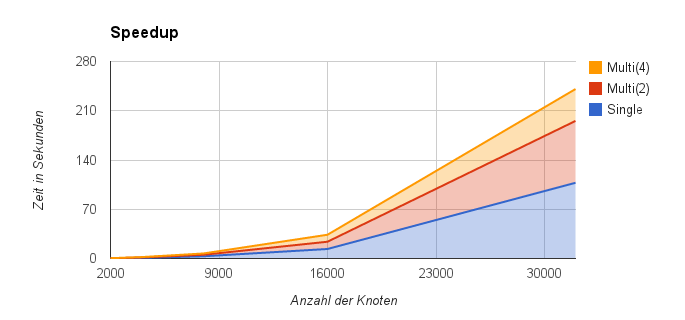
\includegraphics[width=0.8\textwidth]{./daten/speedup_openmp.png}
  \caption{Speedup OpenMP}
  \label{speedup_openmp}
\end{figure}